The second task required us to compute a smooth input state curve and find the optimal trajectory with respect to that. 
\section{Equilibrium computation and quasi-static pair}
The first choice to be made is which smooth curve to use to move between the two equilibrium values. In order to attain a smooth and at least twice derivable curve, namely $x(\cdot) \in \mathit{C}^2$, we decided to use a sigmoid. 
We tuned the parameters to make the curve symmetric with respect to the positive time interval, and to have a slower transition between the values. The desired curve we obtained for $\beta$ and $V$ ended up like:
\begin{equation}
	x(t)= x_{eq}^1  + (x_{eq}^2 - x_{eq}^1) \sigma(\frac{(t-\frac{T}{2})}{4T}) 
\end{equation}
We then obtain the desired curve for the restricted system by finding the quasi-static equilibrium pair for each of the points we found, as previously done in Task 1. This way we end up with the sigmoid desired curve for the velocities. In order to find the desired positions, we integrate them by using the velocities we just found. The final result can be found in figure:
\begin{figure}[!h]
	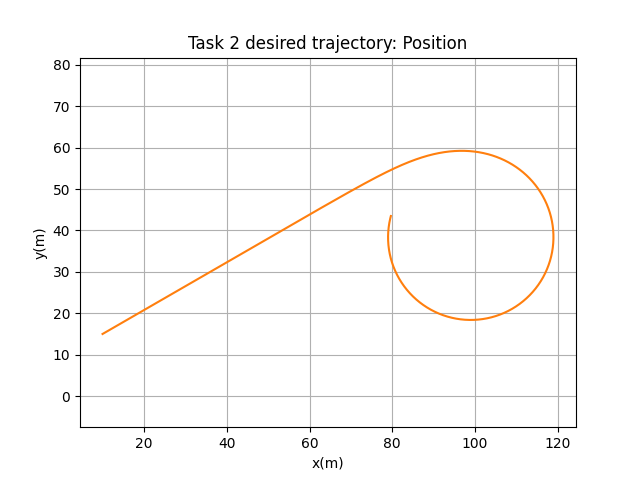
\includegraphics[width=\linewidth]{figs/des_pos_task2.png}
	\caption{Desired smooth position trajectory}
\end{figure} 

\begin{figure}[!h]
	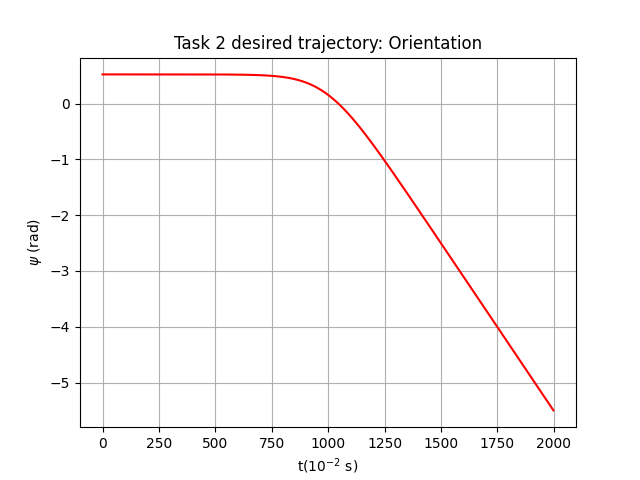
\includegraphics[width=\linewidth]{figs/des_or_task2.png}
	\caption{Desired smooth $\psi$ trajectory}

	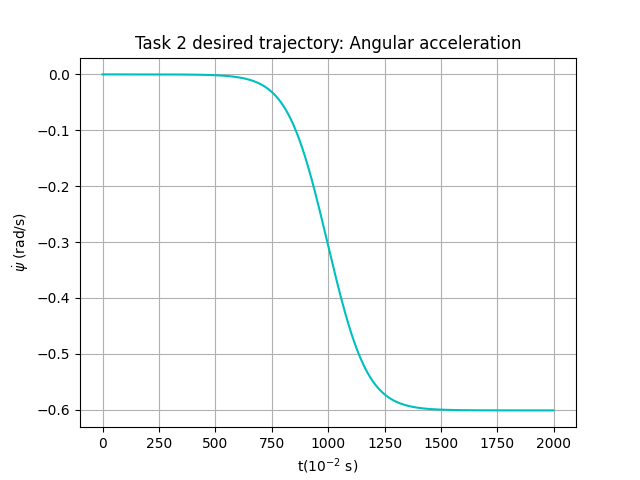
\includegraphics[width=\linewidth]{figs/des_psidot_task2.png}
	\caption{Desired smooth $\dot{\psi}$ trajectory}
	
\end{figure} 

\begin{figure}[!h]
	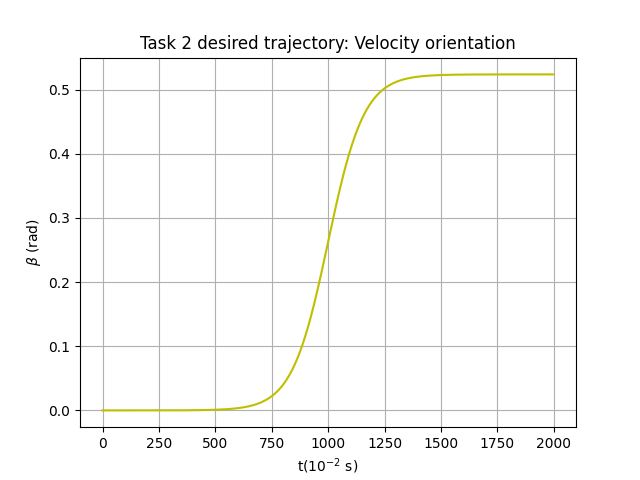
\includegraphics[width=\linewidth]{figs/des_beta_task2.png}
	\caption{Desired smooth $\beta$ trajectory}
	
	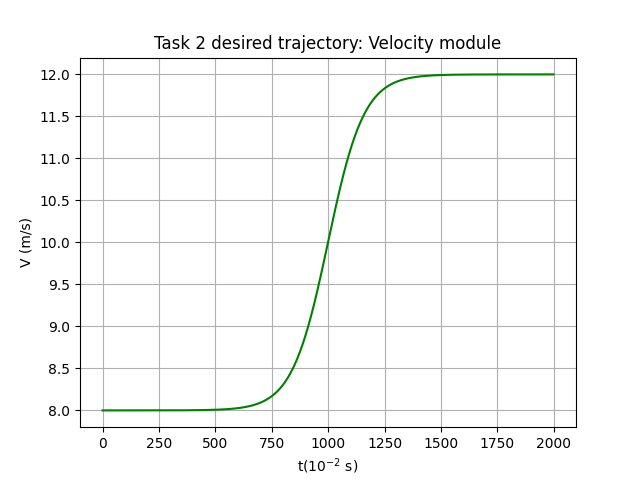
\includegraphics[width=\linewidth]{figs/des_V_task2.png}
	\caption{Desired smooth $V$ trajectory}
\end{figure} 

\FloatBarrier

\section{Newton's method on smooth curve}
We proceded with the Newton's method much in the same way we did for task one. We used the same cost matrices and applied the same routine. In figure the results at different iterations can be found. 

\begin{figure}[!h]
	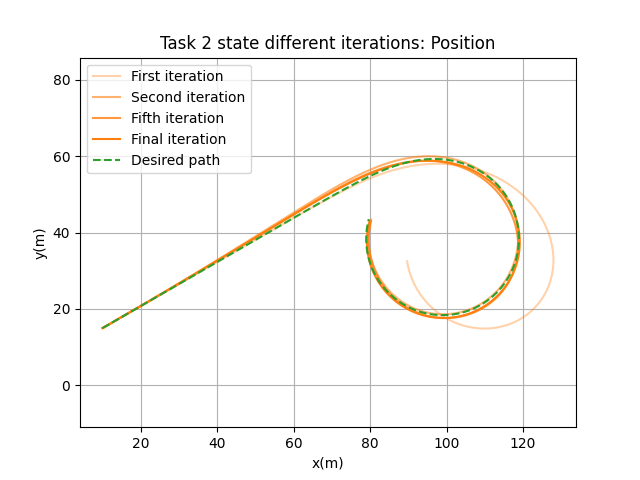
\includegraphics[width=0.5\columnwidth]{figs/positionsk_task2.png}
	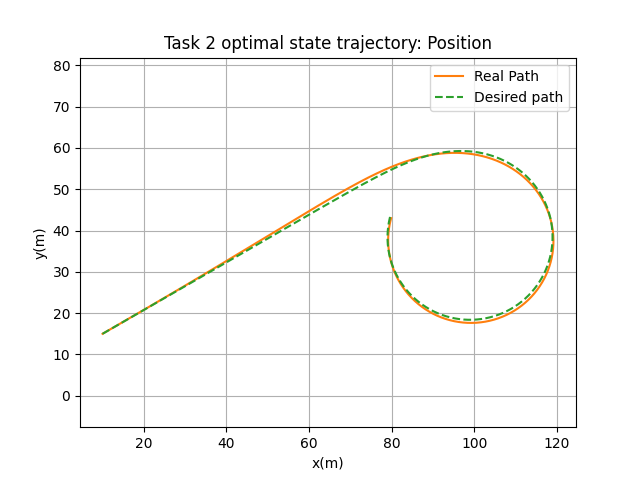
\includegraphics[width=0.5\columnwidth]{figs/onepos_task2.png}
	\caption{Desired smooth position trajectory}
\end{figure} 

\begin{figure}[!h]
	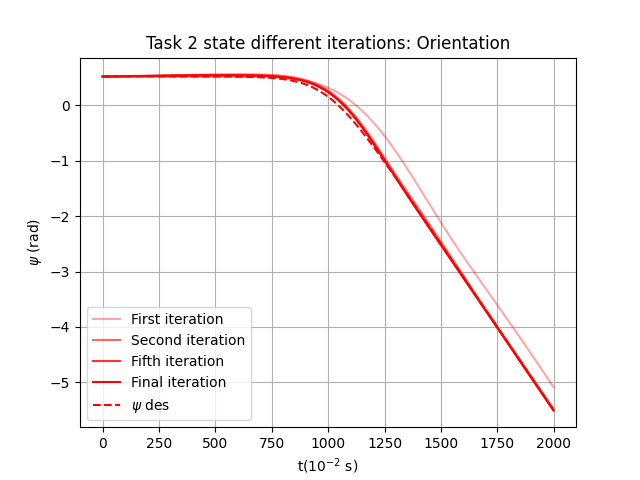
\includegraphics[width=0.5\columnwidth]{figs/orientationsk_task2.png}
	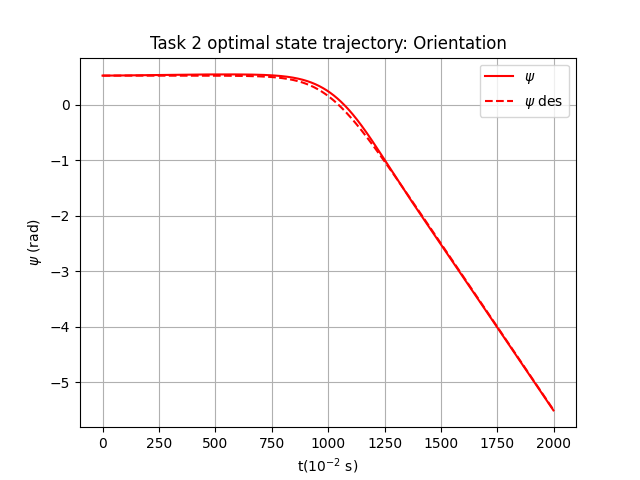
\includegraphics[width=0.5\columnwidth]{figs/oneor_task2.png}
	\caption{Desired smooth position trajectory}
\end{figure} 


\begin{figure}[!h]
	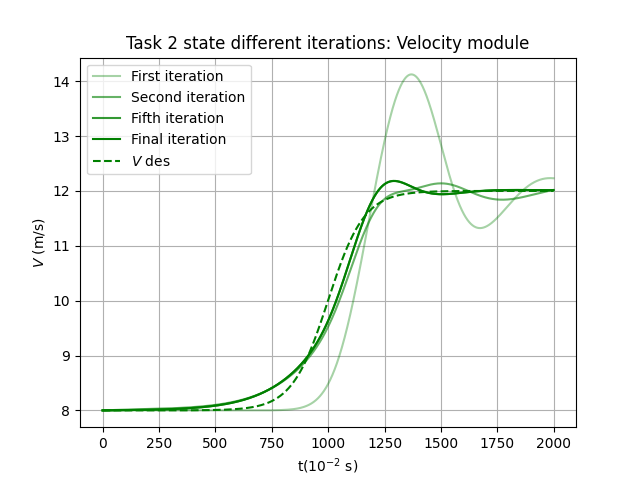
\includegraphics[width=0.5\columnwidth]{figs/velocitiesk_task2.png}
	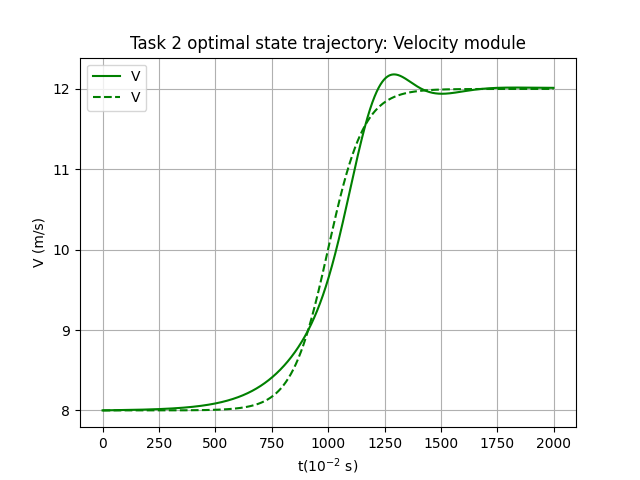
\includegraphics[width=0.5\columnwidth]{figs/oneV_task2.png}
	\caption{Desired smooth position trajectory}
\end{figure} 


\begin{figure}[!h]
	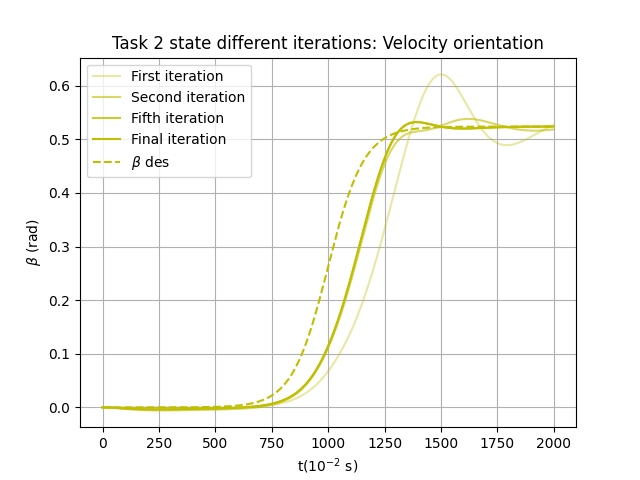
\includegraphics[width=0.5\columnwidth]{figs/betak_task2.png}
	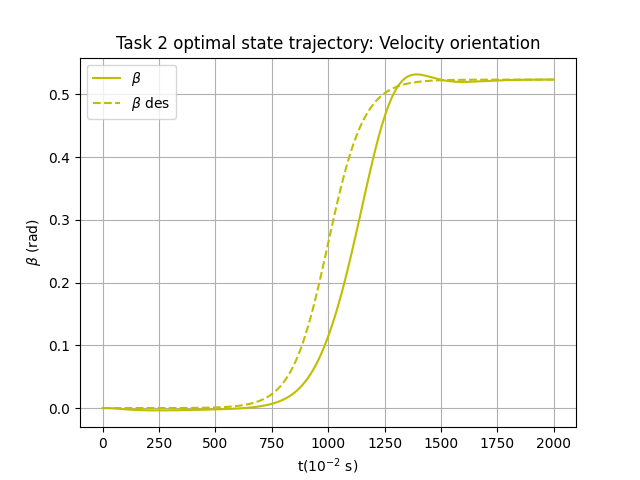
\includegraphics[width=0.5\columnwidth]{figs/onebeta_task2.png}
	\caption{Desired smooth position trajectory}
\end{figure} 


\begin{figure}[!h]
	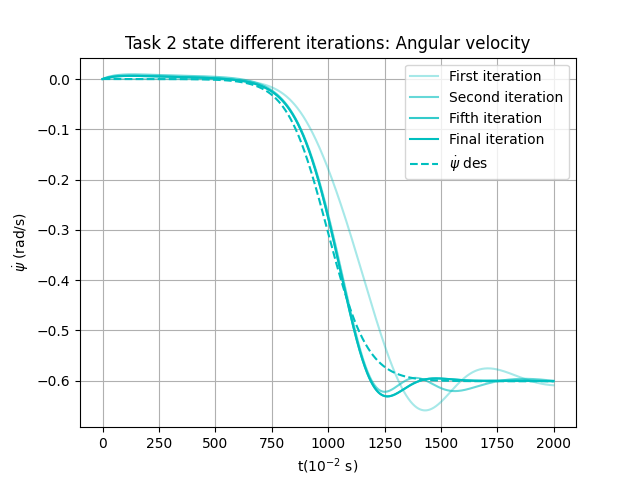
\includegraphics[width=0.5\columnwidth]{figs/psidotk_task2.png}
	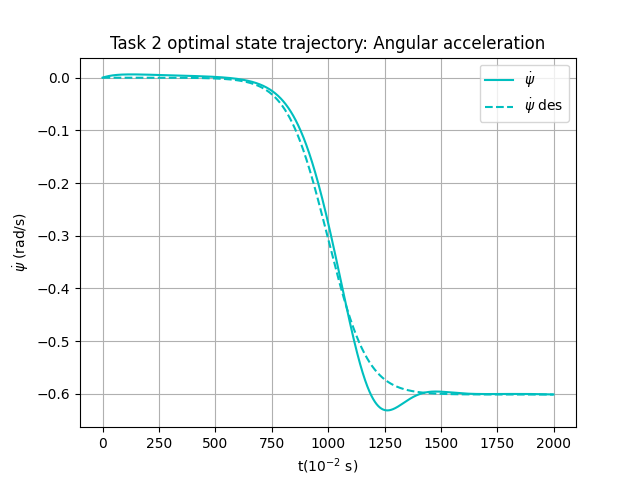
\includegraphics[width=0.5\columnwidth]{figs/onepsidot_task2.png}
	\caption{Desired smooth position trajectory}
\end{figure} 


\begin{figure}[!h]
	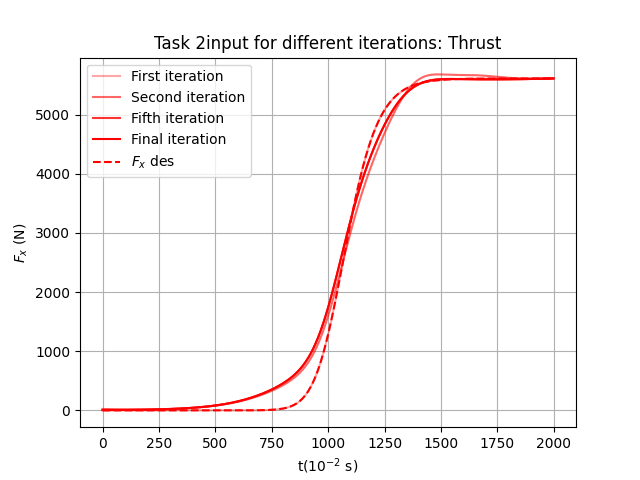
\includegraphics[width=0.5\columnwidth]{figs/Fxk_task2.png}
	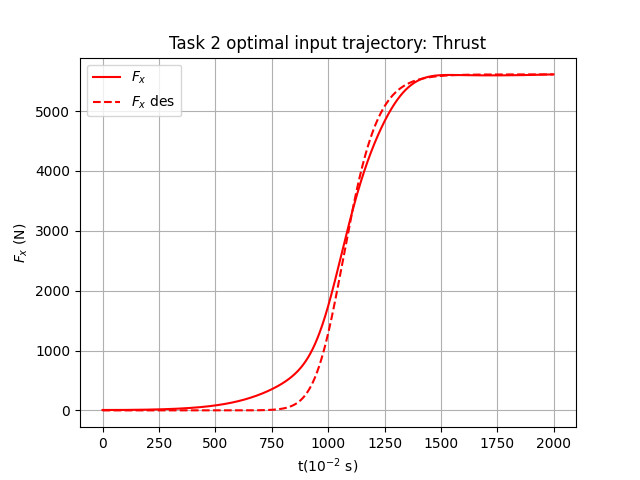
\includegraphics[width=0.5\columnwidth]{figs/Onefx_task2.png}
	\caption{Desired smooth position trajectory}
\end{figure} 


\begin{figure}[!h]
	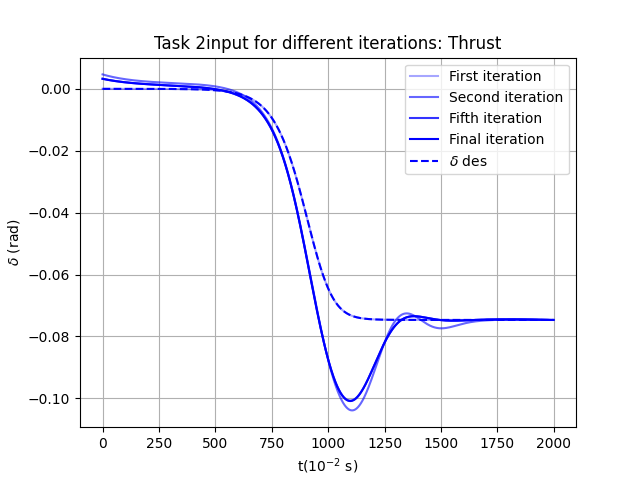
\includegraphics[width=0.5\columnwidth]{figs/deltak_task2.png}
	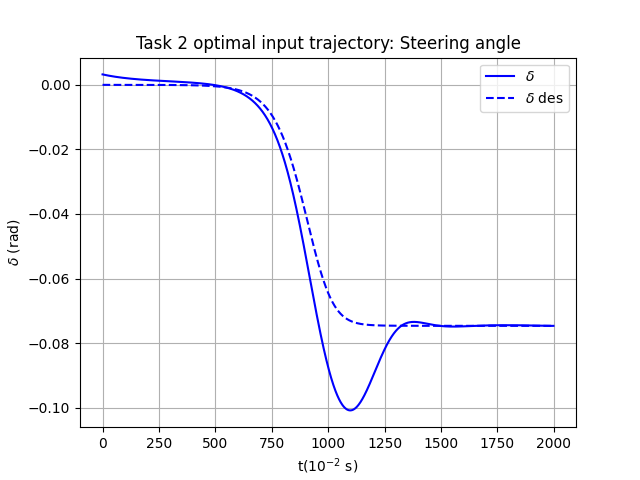
\includegraphics[width=0.5\columnwidth]{figs/onedelta_task2.png}
	\caption{Desired smooth position trajectory}
\end{figure} 


\FloatBarrier

Below are some of the Armijo's plots for the secon task. The plot was taken every two iterations.
\begin{figure}[!h]
	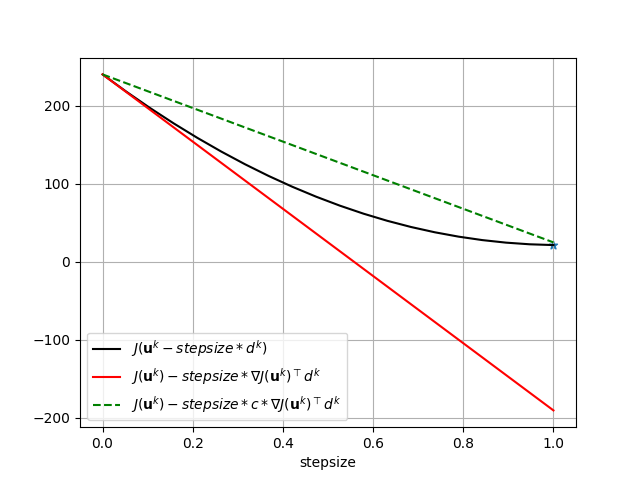
\includegraphics[width=0.5\linewidth]{figs/arm0_task2.png}
	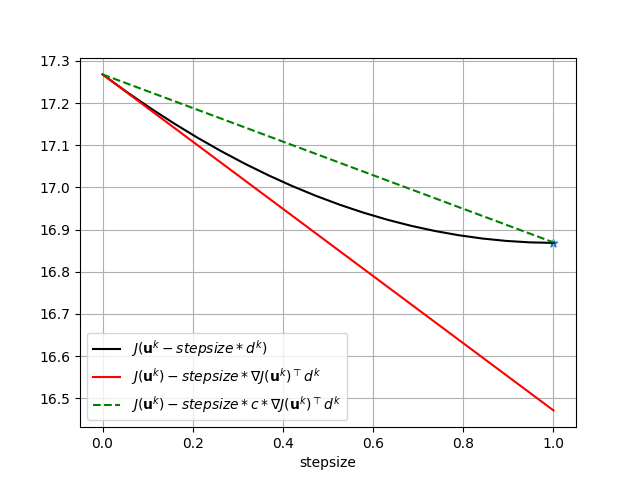
\includegraphics[width=0.5\linewidth]{figs/arm2_task2.png}
	\caption{Armijo's plot at first and third iteration}
\end{figure}
\begin{figure}[!h]
	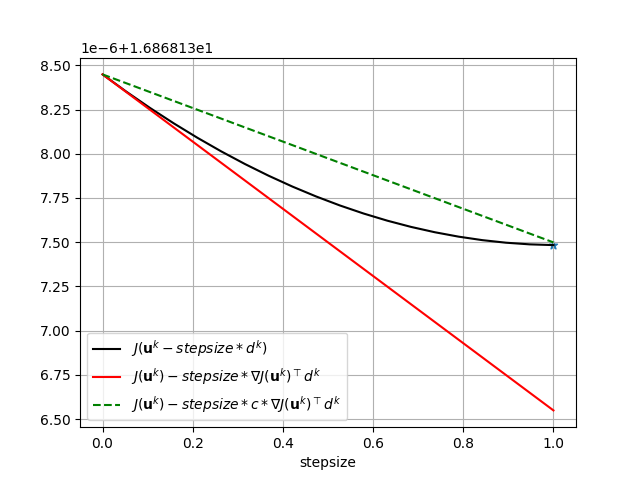
\includegraphics[width=0.5\linewidth]{figs/arm4_task2.png}
	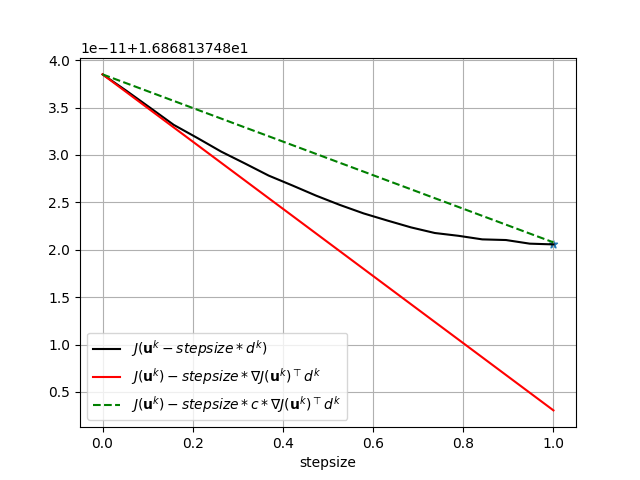
\includegraphics[width=0.5\linewidth]{figs/arm6_task2.png}
	\caption{Armijo's plot at the fifth and last iteration}
\end{figure} 

\FloatBarrier

Lastly, the plots for the cost and gradient norm over iterations can be found here.
\begin{figure}[!h]
	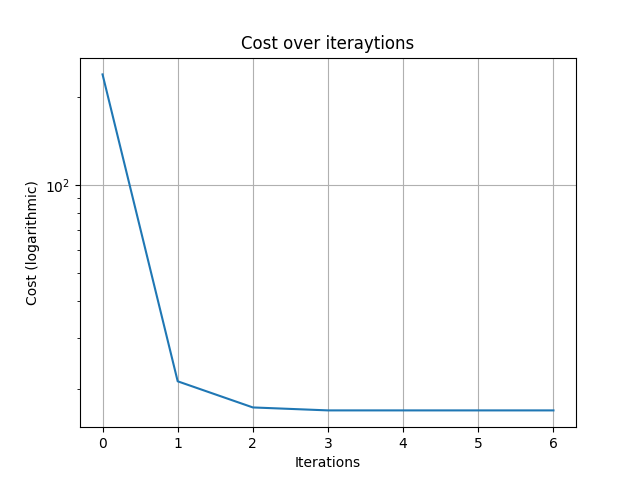
\includegraphics[width=0.5\linewidth]{figs/cost_iter_task2.png}
	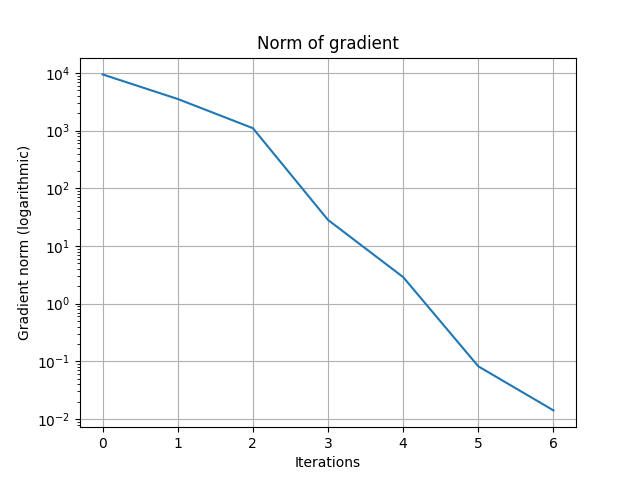
\includegraphics[width=0.5\linewidth]{figs/gradientnorm_task2.png}
	\caption{Armijo's plot at the fifth and last iteration}
\end{figure} 

\section{Conclusions}
The smooth desired curve leads to a nicer trajectory in terms of overshooting and use of the inputs. The overall cost of the trajectory is $16,87$, which is less then a third of the cost for the step trajectory ($54,58$). The inputs don't have discontinuities anymore and, as seen in the plots, stay closer to the desired curve (the quasi-static input curve)than in task one. Overall, we can clearly see the advantage in asking for a smooth input state curve rather than a step. 